\subsection{Three-way scientific evidence reveals class cancellation}
\label{sec:scifact3}
The two-label SciFact check omits the no-information decision an evidence workflow may need. After inspecting that scope gap, we froze a separate, model-blind \emph{follow-up before its own inference}, not before the earlier experiment. From 339 unique official claim--cited-abstract pairs, we selected 60 per class: 138 annotated support, 71 contradiction and 130 cited documents without annotated abstract evidence form the three eligible pools. The 180 selected claims and abstracts are each unique. \textsc{NoInfo} is the source's absence-of-annotation convention, not an independently adjudicated negative. This remains a \emph{cited-document} relation task, not open retrieval or global scientific truth. Four conditions (original, exact repeat, candidate reversal, title removal) yield 720 logical requests per system. Four local adapters passed complete-input checks.

Figure~\ref{fig:scifact3-main} sharpens the paired-accuracy argument. Qwen changes 60/180 semantic labels under reversal and none on exact repeat, yet total reference agreement barely moves, $104/180\to101/180$ ($-1.7$ points; paired 95\% interval $[-7.8,+4.4]$). The net conceals a $54/60\to30/60$ drop on \textsc{NoInfo} ($-40.0$ points; label-stratified interval $[-53.3,-28.3]$) and a $5/60\to18/60$ rise on contradiction ($+21.7$ points; $[+11.7,+31.7]$). All 60 changed labels were base \textsc{NoInfo} predictions: 42 became support and 18 contradiction. This is interface-level sensitivity, not a pure semantic-order effect, because the code-likelihood adapter reassigns answer codes under reversal. Jev changes no labels under reversal, but two on exact repeat; its $148/180$ base-correct cases remain jointly correct. Class-specific turnover is more informative than the small total difference, even in an intentionally balanced sample.

\begin{figure}[H]
\centering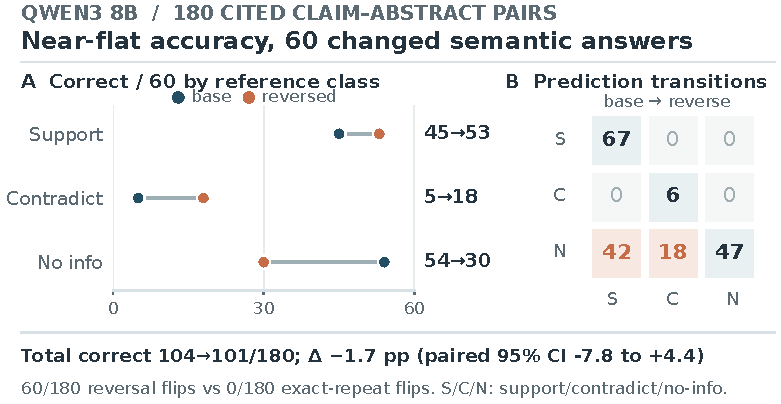
\includegraphics[width=.99\linewidth]{figures/fig_scifact3_compact.pdf}
\caption{Three-class SciFact cited-abstract control for Qwen3 8B. Left: same-pair reference-correct counts by class (60/class); right: all 180 base-to-reversed semantic prediction transitions. S/C/N denote support/contradiction/no-information. Overall accuracy barely moves despite 60 label switches; exact repeat has zero. No-information is an explicitly cited abstract without annotated evidence, not an arbitrary unlabeled corpus pair. Intervals in text use 10,000 paired, label-stratified claim/document-cluster resamples.}
\label{fig:scifact3-main}
\end{figure}

Removing the source-paper title is a different stressor: Laya English changes 60/180 labels and its reference agreement rises from $81/180$ to $100/180$, including $20/60\to39/60$ on \textsc{NoInfo}. The frozen variant removes \texttt{state.paper\_title} while retaining an instruction that mentions the title, creating a minor instruction--state mismatch; a title may also contain evidence. This is neither a semantics-preserving invariance test nor proof of a shortcut. The two-class and three-class SciFact samples have different label spaces and only partial positive-case overlap, so their raw accuracies are not directly comparable. The source/reference and class-stratified audit is retained separately in the companion artifact.

\paragraph{Post-hoc full-census sensitivity.} We reran all five systems on all 339 eligible cited claim--abstract pairs, rather than combining old predictions with new ones. In the 159 pairs outside the earlier balanced three-choice selection, Qwen's reversal reduces \textsc{NoInfo} agreement $60\to38/70$ ($-31.4$ points; paired claim-cluster 95\% interval $[-42.4,-21.1]$); gains on support ($65\to74/78$) and contradiction ($4\to7/11$) partly conceal this as $129\to119/159$ overall (interval $[-13.7,+1.2]$). On all 339, \textsc{NoInfo} is $112\to68/130$ while overall agreement is $231\to220/339$. Figure~\ref{fig:scifact3-census-main} shows the changed reference mix. This same-source, post-hoc check is not an independent holdout: 37 complement positives appeared in the earlier two-choice task. A separately frozen execution-context control adds 6,780 decisions: at most 7/339 predictions move per condition/plan, while Qwen's option-reversal flips remain 95--97 and its \textsc{NoInfo} decline persists (Appendix~\ref{app:scifact3-census}).

\begin{figure}[H]
\centering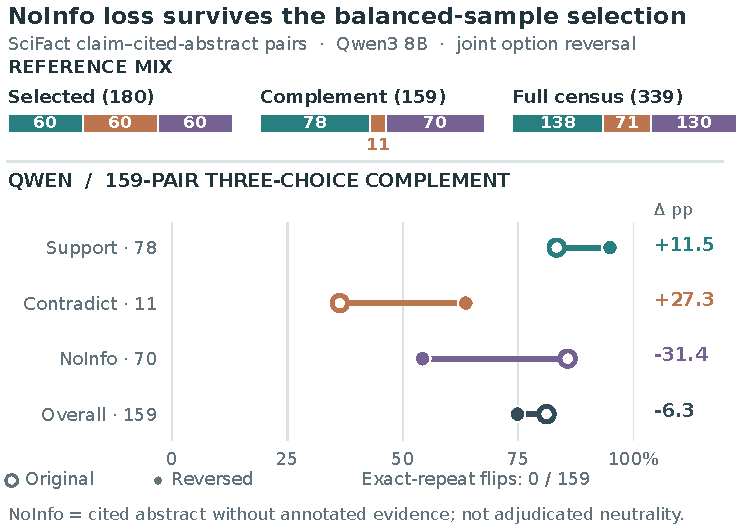
\includegraphics[width=.99\linewidth]{figures/fig_scifact3_census_main.pdf}
\caption{Qwen three-class cited-pair census. The top strip contrasts the deliberately balanced 180 with its 159-pair same-source complement and the full 339. Open/filled points are original/joint-reversal reference agreement from the \emph{fresh full run}; the printed differences are percentage points. NoInfo denotes an explicitly cited abstract without annotated evidence, not adjudicated neutrality. Reversal also remaps answer codes in this adapter; exact repeat yields zero Qwen flips on the complement. Thirty-seven complement positives appeared in the earlier two-choice task.}
\label{fig:scifact3-census-main}
\end{figure}
